\documentclass[]{article}
\usepackage[latin1]{inputenc}
\usepackage{amsmath,amssymb,bm} % math stuff

\usepackage{tikz}
\usetikzlibrary{arrows,calc,positioning,shadows,shapes}


%opening
\title{The guide to Pycle (\textbf{Py}thon \textbf{C}ompresive \textbf{Le}arning toolbox)}
\author{Vincent Schellekens}

\newcommand{\code}{\texttt}
\renewcommand{\Vec}[1]{\bm{#1}} % Pour les vecteurs, re if using amsmath


\begin{document}

% TODO 
% - link to matlab toolbox

\maketitle

\begin{abstract}
	This is the guide to Pycle, a toolbox for Compressive Learning. It is structured as follows: first we shortly explain the theoretical methods this toolbox implements. Then, we explain how the toolbox is structured, and the main steps that a user should follow to use it. The detailed documentation of all the functionalities in the toolbox is then provided, followed by some practical examples to get started easily.
\end{abstract}


\section{What is Compressive Learning?}
% TODO

		
\begin{figure}[!htb]
	\centering
	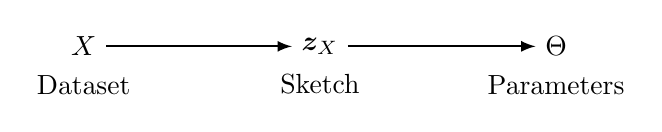
\begin{tikzpicture}
	% Place nodes
	\node [label=below:Dataset] (dataset) at (0,0) {$X$};
	\node [label=below:Sketch] (sketch) at (3,0) {$\Vec{z}_X$};
	\node [label=below:Parameters] (parameters) at (6,0) {$\Theta$};
	
	% Draw edges
	\draw [->, thick, -latex] (dataset) -- (sketch);
	\draw [->, thick, -latex] (sketch) -- (parameters);
	\end{tikzpicture}
	\caption{Compressive learning .}
	\label{fig:CL}
	\end {figure}


See \cite{gribonval2017compressive} for a complete introduction to compressive learning.

\section{An overview of Pycle}
% TODO explain how it is structured, how to use


\subsection{Requirements}
The Pycle package builds on a set of standard Python libraries, that are required to run it:
\begin{itemize}
	\item \code{numpy}
	\item \code{scipy}
\end{itemize}

\subsection{Typical workflow}

A typical use of Pycle follows the following steps:
\begin{enumerate}
	\item Design a sketch operator, then sketch the dataset using the \code{sketching.py} module.
	\item Extract a model from the sketch by a compressive learning method contained in the \code{compressive\_learning.py} module.
\end{enumerate}




	
		
\begin{figure}[!htb]
	\centering
		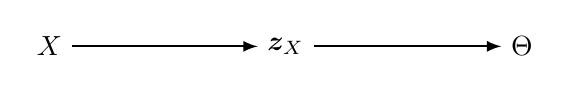
\begin{tikzpicture}
		% Place nodes
		\node (dataset) at (0,0) {$X$};
		\node (sketch) at (3,0) {$\Vec{z}_X$};
		\node (parameters) at (6,0) {$\Theta$};
		
		% Draw edges
		\draw [->, thick, -latex] (dataset) -- (sketch);
		\draw [->, thick, -latex] (sketch) -- (parameters);
		\end{tikzpicture}
	\caption{Flowchart of a typical compressive learning execution with Pycle.}
	\label{fig:flowchart}
\end {figure}
		




\section{Documentation}
\subsection{Sketching methods} 

\subsection{Learning tools} 

\subsection{Utilities} 

\section{Examples}
% TODO some examples, or put notebooks instead?


\newpage
\bibliography{guidebib.bib}
\bibliographystyle{ieeetr}


\end{document}
